%============================================================
\section{Results}
\label{sec:results}
%============================================================
\begin{table*}[t]
\centering
\caption{Main comparison (5-fold patient-grouped CV, pooled out-of-fold predictions on all
\NImages{} images; mean$\pm$s.d.\ over 3 seeds, or 2 seeds for the contrastive rows). The 95\% CI is a
patient-level bootstrap of the seed-averaged predictions. F1 and accuracy use the arg-max class.
Parameters are trainable parameters, excluding the frozen DenseNet.}
\label{tab:main}
\small
\begin{tabular}{@{}lcccccc@{}}
\toprule
Model & macro AUROC & 95\% CI & macro AUPRC & macro F1 & Accuracy & Params (M)\\
\midrule
\tabinput{tables/main.tex}
\bottomrule
\end{tabular}
\end{table*}

\subsection{Fusion helps, provided the text branch is competent}
\Cref{tab:main} and \cref{fig:main} summarise the main comparison. Images alone reach
\AUC{img_only} macro AUROC. Structured data alone reaches \AUC{tab_only}, the masked note alone
\AUC{txt_only}, and note plus structured data \AUC{txt_tab_only}. All three fusion paradigms that
use every modality do better: early fusion \AUC{early_fusion}, IRENE mid fusion (k=2)
\AUC{irene_k2} and late fusion \AUC{late_fusion}. A patient-level paired bootstrap
(\cref{tab:sig}) finds IRENE clearly better than image-only (\SIG{img_only}{diff}, 95\% CI
[\SIG{img_only}{lo}, \SIG{img_only}{hi}]). The gain over note + structured is smaller and
borderline (\SIG{txt_tab_only}{diff}, CI [\SIG{txt_tab_only}{lo}, \SIG{txt_tab_only}{hi}],
$p{=}$\SIG{txt_tab_only}{p}). The differences among the three fusion paradigms are within the
bootstrap uncertainty (IRENE vs.\ early: $p{=}$\SIG{early_fusion}{p}; vs.\ late: $p{=}$\SIG{late_fusion}{p}). Early fusion is also the least stable across seeds
(s.d.\ \AUCsd{early_fusion} against \AUCsd{irene_k2} for IRENE).

One engineering detail mattered more than any architectural choice. In a pilot run, the
note branch was built only from static word vectors, truncated to \MaxTxt{} tokens and trained
from scratch on about 500 notes. The note-only model then reached only about 0.58, and fused models
about 0.71--0.74. A single \emph{document token} fixes this: a TF-IDF$\to$SVD embedding
of the entire note, fitted inside each training fold, plays the role of IRENE's BERT sentence
features. With it and class-balanced BCE, the note-only model rises to \AUC{txt_only} and the
fused models to about 0.78--0.79. \Cref{tab:ablation} isolates the document token
(\AUC{irene_k2_nodoc} without it versus \AUC{irene_k2} with it).

\begin{figure}[t]
\centering
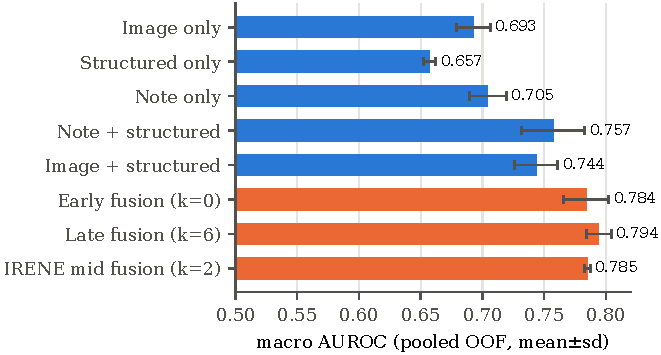
\includegraphics[width=\columnwidth]{figures/main_results.pdf}
\caption{Macro AUROC by input and fusion paradigm. Blue: one or two modalities.
Orange: all three modalities fused. Error bars: s.d.\ over 3 seeds.}
\label{fig:main}
\end{figure}

\begin{table}[t]
\centering
\caption{Patient-level paired bootstrap (1{,}000 resamples) of the macro-AUROC difference
between IRENE (k=2) and other models, using seed-averaged out-of-fold predictions.}
\label{tab:sig}
\small
\setlength{\tabcolsep}{4pt}
\begin{tabular}{@{}lccc@{}}
\toprule
IRENE (k=2) & $\Delta$AUROC & 95\% CI & $p$\\
\midrule
\tabinput{tables/significance.tex}
\bottomrule
\end{tabular}
\end{table}

\begin{table*}[t]
\centering
\caption{Ablations (pooled-OOF macro AUROC and AUPRC, mean$\pm$s.d.\ over seeds). ``No note''
re-evaluates the same model with the note removed at test time. R@5 is image$\to$note retrieval
in \% (chance $\approx$4\%).}
\label{tab:ablation}
\small
\begin{tabular}{@{}lccccc@{}}
\toprule
Variant & macro AUROC & macro AUPRC & AUROC, no note & R@5 & seeds\\
\midrule
\tabinput{tables/ablation.tex}
\bottomrule
\end{tabular}
\end{table*}

\subsection{Where to fuse}
\Cref{fig:fusion} varies the number $k$ of dual-stream blocks with IRENE's bidirectional
attention, keeping depth fixed at $L{=}6$. One or two blocks of cross-modal attention followed
by joint self-attention (k=1: \AUC{irene_k1}; k=2: \AUC{irene_k2}) perform as well as early
fusion. Accuracy then falls as fusion is delayed with cross-attention active (k=3: \AUC{irene_k3};
k=4: \AUC{irene_k4}). It collapses when all six blocks are bidirectional (k=6: \AUC{irene_k6}).
Yet the same depth \emph{without} cross-attention, i.e.\ plain late fusion, is the best model
(\AUC{late_fusion}). The pattern suggests that, on a few hundred training patients, the
extra cross-attention parameters (\cref{tab:main}) and the repeated mixing of a noisy note
into the image stream cause overfitting rather than useful alignment. IRENE's choice of shallow
cross-modal attention followed by joint layers is a sensible point on this curve. The
original paper, with about 10$\times$ more patients, did not report this sweep.

\begin{figure*}[t]
\centering
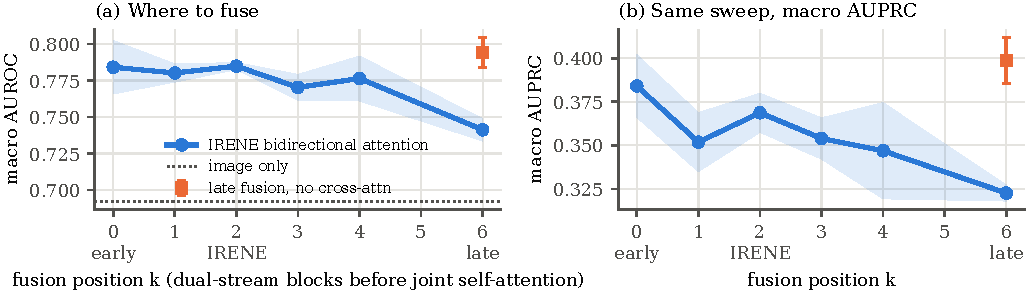
\includegraphics[width=\textwidth]{figures/fusion_position.pdf}
\caption{Fusion position. $k$ dual-stream IRENE blocks are followed by $6-k$ joint blocks;
$k{=}0$ is early fusion. Orange square: $k{=}6$ without cross-attention (late fusion). Dotted
line: image only. Shaded bands and error bars: $\pm$1 s.d.\ over seeds.}
\label{fig:fusion}
\end{figure*}

\subsection{How the streams attend to each other}
\Cref{fig:attn} fixes $k{=}2$ and changes only the combination rule. IRENE's average of self-
and cross-attention (\AUC{irene_k2}) matches the unidirectional variants (image$\to$text
\AUC{attn_i2t}, text$\to$image \AUC{attn_t2i}) and the no-exchange control (\AUC{attn_none}).
It clearly beats ViLBERT-style co-attention, which drops self-attention in the dual-stream
blocks (\AUC{attn_bi_cross}). Flamingo-style tanh gates (\AUC{attn_gated}) are the least
stable across seeds (s.d.\ \AUCsd{attn_gated}). The practical conclusion is that each stream
must keep its intra-modal self-attention. Cross-attention in the first blocks is not harmful,
but at this data scale the joint self-attention layers can recover most of what it provides.
\Cref{fig:attn}b repeats the evaluation with the note removed. All variants fall to 0.58--0.61,
which shows that the models rely heavily on the note whatever the attention structure.

\begin{figure*}[t]
\centering
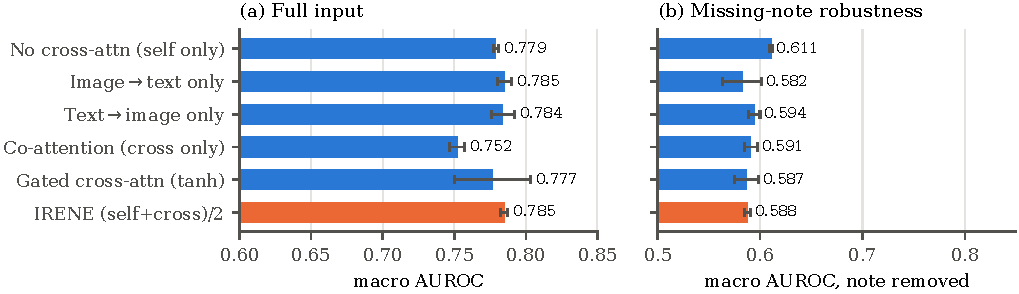
\includegraphics[width=\textwidth]{figures/attention_structure.pdf}
\caption{Attention structure inside the $k{=}2$ dual-stream blocks. (a) Full input.
(b) The same trained models evaluated with the clinical note removed.}
\label{fig:attn}
\end{figure*}

\subsection{Image--text contrastive learning}
\Cref{fig:contrastive} adds a CLIP or SigLIP loss on unimodal pooled embeddings. For IRENE
(k=2), both objectives \emph{lower} diagnostic AUROC, and more so as $\lambda$ grows (CLIP:
\AUC{clip_l0.1}, \AUC{clip_l0.5}, \AUC{clip_l1.0}; SigLIP: \AUC{siglip_l0.1}, \AUC{siglip_l0.5},
\AUC{siglip_l1.0}). SigLIP degrades more gracefully than CLIP. Retrieval is above chance but
modest (R@5 \RFIVE{clip_l0.5}\% for CLIP at $\lambda{=}0.5$, against about 4\% for chance). The
picture changes for late fusion. The two encoders are then separate, so the model is a CLIP-style
dual encoder with a classification head. Alignment leaves AUROC unchanged (\AUC{late_clip_l0.5}
against \AUC{late_fusion}) and gives the best retrieval (R@5 \RFIVE{late_clip_l0.5}\%). In the
early-fusion model the aligned embeddings sit at the token level, and alignment reaches
\AUC{early_clip_l0.5}.

Two properties of this dataset explain the weak benefit. First, there are only about 500
training pairs per fold, and many images of the same patient share one note, so the effective
number of distinct pairs is small. Second, the notes describe history and radiographic findings
in heterogeneous styles, with no one-to-one correspondence to the image. Contrastive
pre-training works at the scale of hundreds of thousands to millions of report pairs
\citep{zhang2022convirt,you2023cxrclip,zhang2023biomedclip}. As an auxiliary loss on hundreds
of pairs, it competes with the supervised objective for the shared parameters in the
dual-stream blocks, which is why it hurts mid fusion but not a dual encoder.

\begin{figure*}[t]
\centering
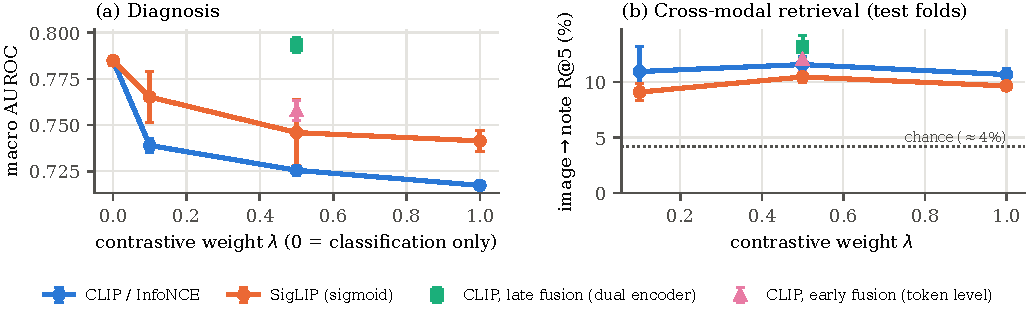
\includegraphics[width=\textwidth]{figures/contrastive.pdf}
\caption{Contrastive alignment. (a) Diagnostic macro AUROC as a function of the alignment
weight $\lambda$ ($\lambda{=}0$ is IRENE without alignment). (b) Image$\to$note Recall@5 on
the test folds.}
\label{fig:contrastive}
\end{figure*}

\subsection{Per-class behaviour}
\Cref{fig:perclass,fig:roc} break results down by class. Compared with the image-only model, fusion gains the most for
COVID-19 (IRENE \PC{irene_k2}{0} vs.\ \PC{img_only}{0}), bacterial pneumonia
(\PC{irene_k2}{2} vs.\ \PC{img_only}{2}) and unspecified pneumonia (\PC{irene_k2}{4} vs.\
\PC{img_only}{4}). The note-based models are strong on exactly these classes (note + structured:
\PC{txt_tab_only}{0}, \PC{txt_tab_only}{2}, \PC{txt_tab_only}{4}). The image contributes more for
fungal pneumonia (image-only \PC{img_only}{3} vs.\ note + structured \PC{txt_tab_only}{3}), where
fusion combines both (\PC{irene_k2}{3}). Tuberculosis and no finding (18 images each) remain the
hardest and noisiest classes for every model.

\begin{figure}[t]
\centering
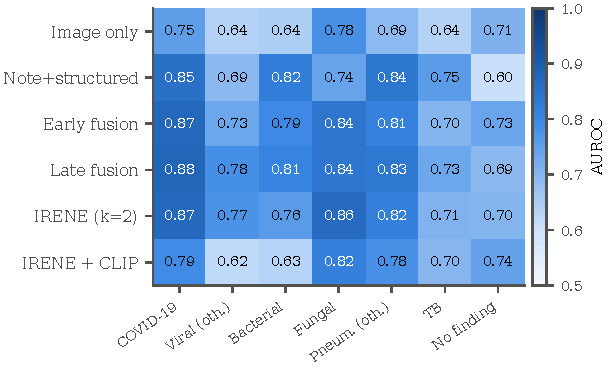
\includegraphics[width=\columnwidth]{figures/per_class.pdf}
\caption{Per-class AUROC (pooled OOF, mean over seeds).}
\label{fig:perclass}
\end{figure}

\begin{figure*}[t]
\centering
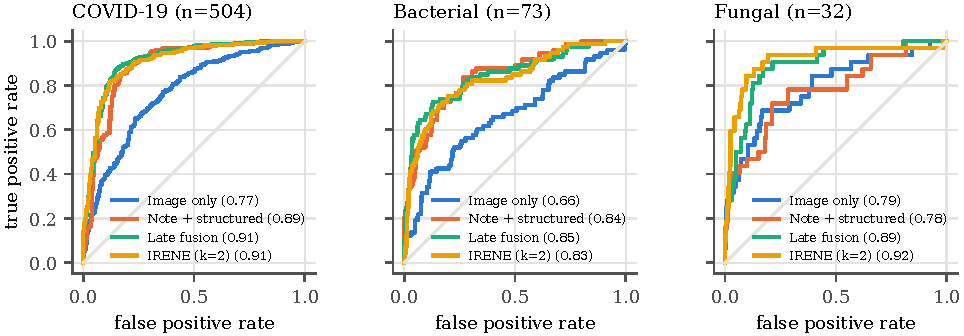
\includegraphics[width=\textwidth]{figures/roc.pdf}
\caption{Pooled out-of-fold ROC curves (seed-averaged predictions) for three classes;
AUROC in the legend.}
\label{fig:roc}
\end{figure*}

\subsection{Label leakage and dataset confounding}
\label{sec:leak}
\begin{table}[t]
\centering
\caption{Shortcut probes. Macro AUROC on all \NImages{} images and on the \NMixed{} images from the
two case repositories that contain \emph{both} COVID-19 and non-COVID cases (Radiopaedia,
Eurorad), where the source cannot identify the label. Logistic regressions use the same folds.}
\label{tab:reference}
\small
\setlength{\tabcolsep}{4pt}
\begin{tabular}{@{}lcc@{}}
\toprule
Model & all images & mixed-source subset\\
\midrule
\tabinput{tables/reference.tex}
\bottomrule
\end{tabular}
\end{table}

\paragraph{Diagnosis terms in notes.} \PctMasked\% of the notes name the diagnosis or the
pathogen. Leaving these terms unmasked raises note + structured from \AUC{txt_tab_only} to
\AUC{txt_tab_only_rawtext} and IRENE from \AUC{irene_k2} to \AUC{irene_k2_rawtext}
(\cref{fig:robust}a). The gain is smaller than one might expect, because the remaining text is
itself highly predictive. A TF-IDF logistic regression on the \emph{masked} notes reaches
\CL{tfidf_masked}, almost as high as on raw notes (\CL{tfidf_raw}), and above every transformer
in this study (\cref{tab:reference}). Masking is still necessary for a fair evaluation, but it is
far from sufficient.

\paragraph{Source confounding.} Public COVID-19 collections gather cases from sources that
differ systematically in their label mix. Some are almost entirely COVID-19 (the SIRM archive,
GitHub-hosted hospital releases, NEJM case reports), while others are mostly non-COVID
(Eurorad). A logistic regression that sees \emph{only} the host of the source URL reaches
\CL{source_only} macro AUROC, on par with the fusion transformers. The notes and the view
(\CL{view_only}) carry this signal implicitly through writing style, translation artefacts
and acquisition protocol. As a de-confounded check, we recompute every metric on the \NMixed{}
images from Radiopaedia and Eurorad, the two repositories that host both COVID-19 and
non-COVID cases. There the source-only probe falls to chance (\CL{source_only@mixed}). The fused models
lose about 6 points and the image-only model about 3, but the ranking is preserved (\cref{tab:reference}). Late fusion
(\MIX{late_fusion}), early fusion (\MIX{early_fusion}) and IRENE (\MIX{irene_k2}) remain above
note + structured (\MIX{txt_tab_only}) and image-only (\MIX{img_only}). The TF-IDF note model is
still the strongest (\CL{tfidf_masked@mixed}). This agrees with the radiograph shortcuts reported
by DeGrave et al.\ \citep{degrave2021shortcuts} and argues for reporting a de-confounded subset
alongside headline numbers on public COVID-19 data.

\begin{figure*}[t]
\centering
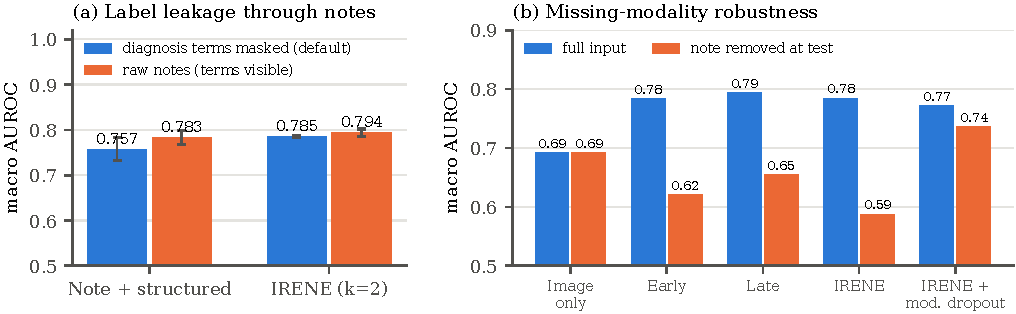
\includegraphics[width=\textwidth]{figures/robustness.pdf}
\caption{(a) Effect of masking diagnosis and pathogen names in the notes (2 seeds for the
raw-note runs). (b) Macro AUROC with the full input and with the note removed at test time.
Modality dropout ($p{=}0.3$) during training closes most of the gap.}
\label{fig:robust}
\end{figure*}

\paragraph{Missing notes.} Deployed systems will not always have a note. When it is removed at
test time, IRENE falls from \AUC{irene_k2} to \NT{irene_k2}, well below the image-only model
(\AUC{img_only}). Early and late fusion degrade less (\NT{early_fusion} and \NT{late_fusion};
\cref{fig:robust}b). The fused models have learned to rely on the note and do not fall back on
the image features. This matches the fragility reported by Ma et al.\ \citep{ma2022missing}.
Training with modality dropout ($p{=}0.3$) raises the no-note AUROC to \NT{irene_k2_moddrop},
close to the image + structured model (\AUC{img_tab}), at a small cost with full input
(\AUC{irene_k2_moddrop}). For a clinical deployment where the note is not always available,
this trade-off is clearly worthwhile.


\subsection{Throughput of the training stack}
\label{sec:throughput}
\begin{figure*}[t]
\centering
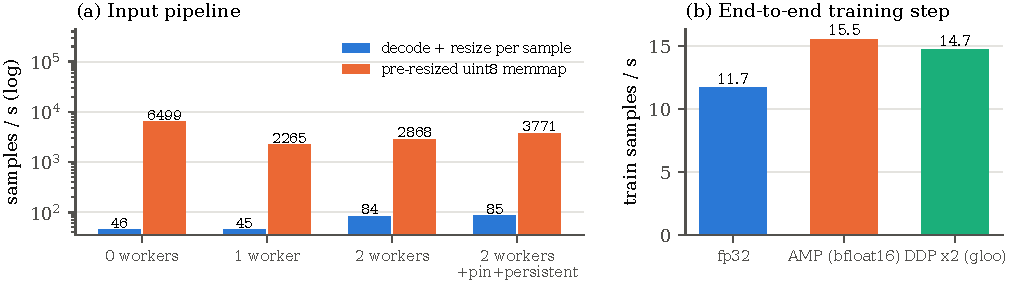
\includegraphics[width=\textwidth]{figures/throughput.pdf}
\caption{Throughput on the 2-core CPU machine used for all experiments. (a) Input pipeline:
decoding and resizing the original radiographs per sample, versus a pre-resized uint8
memory-mapped cache, for several \texttt{DataLoader} settings. (b) One end-to-end training step
of pixel-input IRENE-MM (batch 16), in fp32, with bf16 autocast, and with DDP over 2 Gloo
processes (1 thread each).}
\label{fig:throughput}
\end{figure*}

\Cref{fig:throughput} reports the engineering measurements we could make without a GPU.
Many source radiographs are large JPEG/PNG files, and decoding and resizing them for every
sample limits the input pipeline to \TpDecodeZero{} samples/s in the main process. Two worker
processes help ($\times$\TpWorkerSpeedup{}, \TpDecodeBest{} samples/s). Pre-resizing once into a
memory-mapped uint8 array takes \TpCacheSec{}\,s and raises throughput to \TpMmapBest{}
samples/s ($\times$\TpSpeedup{}). With so little per-sample work on 2 cores, worker processes
then \emph{reduce} throughput because of inter-process transfer. The right
\texttt{num\_workers} depends on the per-sample cost, and should be measured rather than set
by habit. Persistent workers avoid re-forking at every epoch and help consistently when
workers are used. For the model, bf16 autocast raises end-to-end training throughput from
\TpFp{} to \TpAmp{} samples/s on this CPU. DDP with two single-threaded Gloo ranks reaches
\TpDDP{} samples/s, against \TpFp{} for one process with two threads. The same \texttt{train.py}
runs unchanged with NCCL and fp16 loss scaling on GPUs, but we could not measure GPU
utilisation here and make no claim about it.

